\section{Konzeption}

\subsection{Anforderungen}

\subsubsection{Software-Qualitätsmodelle}

\newparagraph{Qualitätsmodell nach McCall}

\newparagraph{ISO/IEC 9126}

\newparagraph{ISO/IEC 25010}


\vspace{1em}
\begin{minipage}{\linewidth}
	\centering
	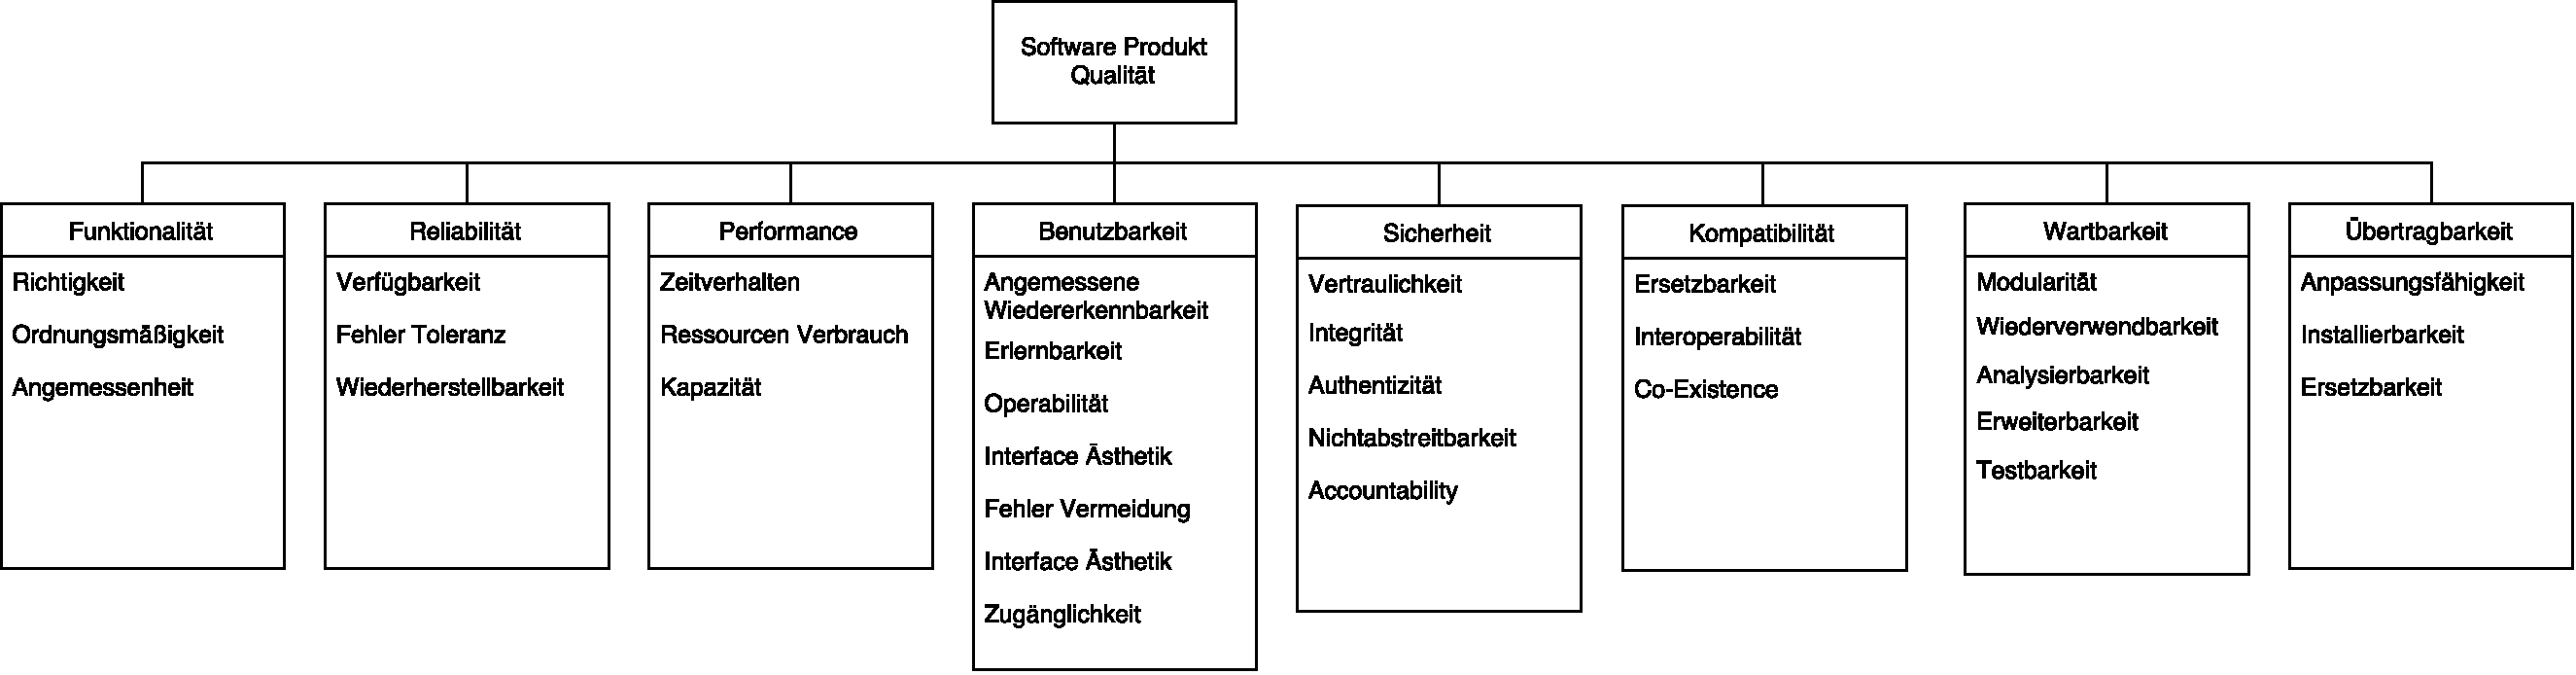
\includegraphics[width=0.9\linewidth]{Konzeption/Bilder/ISO25010_Modell.pdf}
	\captionof{figure}[ISO/IEC 25010 Qualitätsmodell]{ISO/IEC 25010 Software Produkt Qualitätsmodell}
	\label{fig:iso25010}
\end{minipage}

\vspace{1em}
\begin{minipage}{\linewidth}
	\centering
	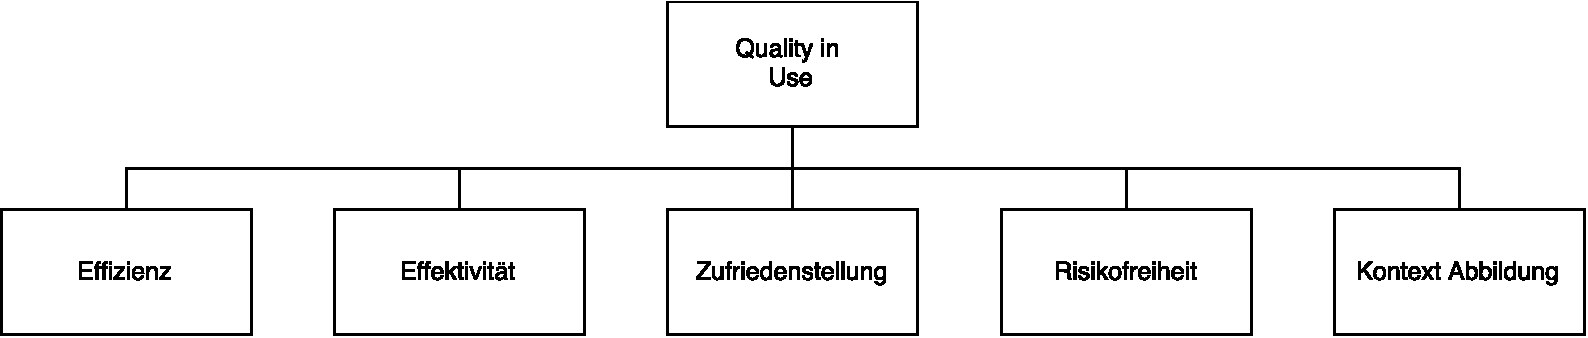
\includegraphics[width=0.9\linewidth]{Konzeption/Bilder/QualityInUse.pdf}
	\captionof{figure}[ISO/IEC 25010 Quality in use]{ISO/IEC 25010 Quality in use model}
	\label{fig:iso25010qiu}
\end{minipage}
 
\subsubsection{Analyse und Wahl der Anforderungen}


\newparagraph{Funktionalität}

\newparagraph{Reliabilität}

\newparagraph{Performance}

\newparagraph{Benutzbarkeit}

\newparagraph{Sicherheit}

\newparagraph{Kompatibilität}

\newparagraph{Wartbarkeit}

\newparagraph{Übertragbarkeit} 
 
\pagebreak
 
\subsection{Evaluation}

\subsubsection{Evaluationsmethoden}

\subsubsection{Wahl der Evalutationsmethoden}

\newparagraph{Subjektive Evaluation}

\newsubparagraph{Cognitive Walkthrough}

\newparagraph{Objektive Evaluation}

\newsubparagraph{Performance Messung}
 
\pagebreak

\subsection{Wahl der Frameworks}

\subsubsection{Spring}

\subsubsection{Vert.X}

\subsubsection{NodeJS}

\subsubsection{Go}